\documentclass{article}

\usepackage{a4wide}
\usepackage{amsmath,bm}
\usepackage{tikz}
\usepackage{3dplot}

\newcommand{\td}{\mathrm{d}}

\begin{document}

\section{General -- state of the art}

We construct numerical quadrature to evaluate the weakly singular integral
%
\begin{equation}
\int_X
\int_Y
\frac{1}{r}
\td \bm{\eta}
\td \bm{\xi}
\quad
r = |\bm{\eta}-\bm{\xi}|
\end{equation}
%
where $X$ and $Y$ denote 2D simplex domains in the same coordinate system.


We first introduce the coordinate difference variable $\bm{\mu} = \bm{\eta}-\bm{\xi}$.
By replacing coordinate $\bm{\eta}$ to the difference, we map the integration domain $Y$ into the difference domain $M$, where the singularity can be cancelled:
%
\begin{equation}
\int_X
\int_{M(\bm{\xi})}
\frac{1}{|\bm{\mu}|}
\td \bm{\mu}
\td \bm{\xi}
\end{equation}
%
The integration domain $M$ of the internal integral depends on the outer integral variable $\bm{\xi}$ as $M(\bm{\xi}) = Y - \bm{\xi}$. In order to define quadratures in the difference domain $M$, the order of integration is exchanged:
%
\begin{equation}
\int_{M}
\frac{1}{|\bm{\mu}|}
\int_{X(\bm{\mu})}
\td \bm{\xi}
\td \bm{\mu}
\end{equation}
%
where
%
\begin{equation}
M = \bigcup M(\bm{\xi}),
\qquad
X({\bm{\mu}}) = (-\bm{\mu} + Y) \cap X
\end{equation}

Now the quadrature is defined by
\begin{itemize}
	\item splitting the domain $M$ into non overlapping subdomains,
	\item defining an appropriate (regular or singular) 2D outer quadrature for each subdomain.
	\item defining a regular 2D internal quadrature over the domain $X(\bm{\mu})$ for each quadrature point $\bm{\mu}$ of the outer quadrature
	\item combine the outer and inner quadratures using the rule $\bm{\eta} = \bm{\mu} + \bm{\xi}$
\end{itemize}



\begin{equation}
{\color{blue}\bm{\xi}} = -\bm{\mu} + {\color{red}\bm{\eta}}
\end{equation}



\subsection{tria}

\newcommand{\commontri}{
\path [draw=gray] (1,0) -- (1,1) -- (0,1) -- (-1,0) -- (-1,-1) -- (0,-1) -- cycle;
\path [draw=gray] (-1,0) -- (1,0);
\path [draw=gray] (0,-1) -- (0,1);
\path [draw=gray] (-1,-1) -- (1,1);
\path [draw, ->] (-.2,0) -- (1.2,0) node [anchor = west] {$\xi_1$};
\path [draw, ->] (0,-.2) -- (0,1.2) node [anchor = south] {$\xi_2$};
\path [fill=red, opacity=.5] (0-\m,0-\p) -- (1-\m,0-\p) -- (1-\m,1-\p) -- cycle;
\path [fill = blue, opacity=.5] (0,0) -- (1,0) -- (1,1) -- cycle;
\path [draw, fill] (\m,\p) circle(.03) -- (-\m,-\p) circle(.03);
}


\subsubsection{Domain I.}
%
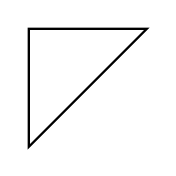
\begin{tikzpicture}[scale=1.5]
\def\m{-.5}
\def\p{-.3}
\commontri
\path [draw, thick] (0,0) -- (-1,0) -- (-1,-1) -- cycle;
\end{tikzpicture}
%
\begin{align}
-\mu_1 &< \xi_1 < 1 \nonumber \\
-\mu_2 &< \xi_2 < -\mu_2 + \xi_1+\mu_1 \nonumber
\end{align}


\subsubsection{Domain II.}
%
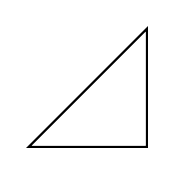
\begin{tikzpicture}[scale=1.5]
\def\m{.6}
\def\p{.3}
\commontri
\path [draw, thick] (0,0) -- (1,0) -- (1,1) -- cycle;
\end{tikzpicture}
%
\begin{align}
0 &< \xi_1 < 1-\mu_1 \nonumber \\
0 &< \xi_2 < \xi_1 \nonumber
\end{align}



\subsubsection{Domain III.}
%
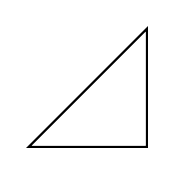
\begin{tikzpicture}[scale=1.5]
\def\m{-.3}
\def\p{.5}
\commontri
\path [draw, thick] (0,0) -- (0,1) -- (-1,0) -- cycle;
\end{tikzpicture}
%
\begin{align}
\mu_2-\mu_1 &< \xi_1 < 1 \nonumber \\
0 &< \xi_2 < \xi_1 - \mu_2+\mu_1\nonumber
\end{align}




\subsubsection{Domain IV.}
%
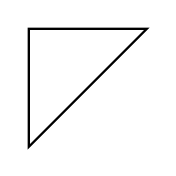
\begin{tikzpicture}[scale=1.5]
\def\m{.3}
\def\p{-.5}
\commontri
\path [draw, thick] (0,0) -- (0,-1) -- (1,0) -- cycle;
\end{tikzpicture}
%
\begin{align}
-\mu_2 &< \xi_1 < 1-\mu_1 \nonumber \\
-\mu_2 &< \xi_2 < \xi_1 \nonumber
\end{align}



\subsubsection{Domain V.}
%
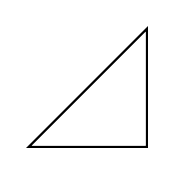
\begin{tikzpicture}[scale=1.5]
\def\m{-.3}
\def\p{-.6}
\commontri
\path [draw, thick] (0,0) -- (-1,-1) -- (0,-1) -- cycle;
\end{tikzpicture}
%
\begin{align}
-\mu_2 &< \xi_1 < 1 \nonumber \\
-\mu_2 &< \xi_2 < \xi_1 \nonumber
\end{align}


\subsubsection{Domain VI.}
%
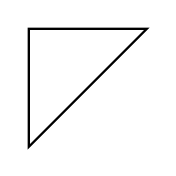
\begin{tikzpicture}[scale=1.5]
\def\m{.3}
\def\p{.6}
\commontri
\path [draw, thick] (0,0) -- (1,1) -- (0,1) -- cycle;
\end{tikzpicture}
%
\begin{align}
\mu_2-\mu_1 &< \xi_1 < 1-\mu_1 \nonumber \\
0 &< \xi_2 < \xi_1 - \mu_2+\mu_1\nonumber
\end{align}



\subsection{quad}

\newcommand{\commonquad}{
\path [draw=gray] (1,-1) -- (1,1) -- (-1,1) -- (-1,-1) -- cycle;
\path [draw=gray] (-1,0) -- (1,0);
\path [draw=gray] (0,-1) -- (0,1);
\path [draw, ->] (-1.2,0) -- (1.2,0) node [anchor = west] {$\xi_1$};
\path [draw, ->] (0,-1.2) -- (0,1.2) node [anchor = south] {$\xi_2$};
\path [fill=red, opacity=.5] (0-\m,0-\p) -- (1-\m,0-\p) -- (1-\m,1-\p) -- (0-\m,1-\p) -- cycle;
\path [fill = blue, opacity=.5] (0,0) -- (1,0) -- (1,1) -- (0,1) -- cycle;
\path [draw, fill] (\m,\p) circle(.03) -- (-\m,-\p) circle(.03);
}



\subsubsection{Domain I.}
%
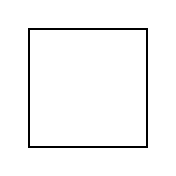
\begin{tikzpicture}[scale=1.5]
\def\m{-.3}
\def\p{-.6}
\commonquad
\path [draw, thick] (0,0) -- (-1,0) -- (-1,-1) -- (0,-1) -- cycle;
\end{tikzpicture}
%
\begin{align}
-\mu_1 &< \xi_1 < 1 \nonumber \\
-\mu_2 &< \xi_2 < 1 \nonumber
\end{align}



\subsubsection{Domain II.}
%
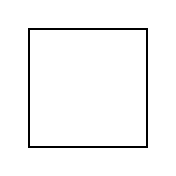
\begin{tikzpicture}[scale=1.5]
\def\m{.3}
\def\p{.6}
\commonquad
\path [draw, thick] (0,0) -- (1,0) -- (1,1) -- (0,1) -- cycle;
\end{tikzpicture}
%
\begin{align}
0 &< \xi_1 < 1 - \mu_1 \nonumber \\
0 &< \xi_2 < 1 - \mu_2 \nonumber
\end{align}


\subsubsection{Domain III.}
%
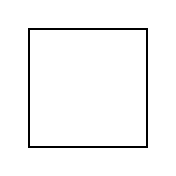
\begin{tikzpicture}[scale=1.5]
\def\m{-.3}
\def\p{.6}
\commonquad
\path [draw, thick] (0,0) -- (-1,0) -- (-1,1) -- (0,1) -- cycle;
\end{tikzpicture}
%
\begin{align}
-\mu_1 &< \xi_1 < 1 \nonumber \\
0 &< \xi_2 < 1- \mu_2 \nonumber
\end{align}


\subsubsection{Domain IV.}
%
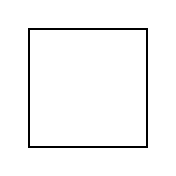
\begin{tikzpicture}[scale=1.5]
\def\m{.3}
\def\p{-.6}
\commonquad
\path [draw, thick] (0,0) -- (1,0) -- (1,-1) -- (0,-1) -- cycle;
\end{tikzpicture}
%
\begin{align}
0 &< \xi_1 < 1-\mu_1 \nonumber \\
-\mu_2 &< \xi_2 < 1 \nonumber
\end{align}


\section{Edge match}

\subsection{Edge match with two rectangles}

The case where coincident square elements share a common edge is displayed  below. It is assumed that the common edge lies on the $\xi_1$ and $\eta_1$ local axes of the two elements, respectively.

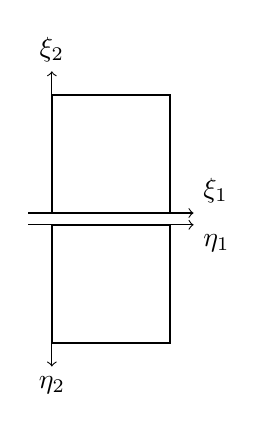
\begin{tikzpicture}[scale=1.5]
\def\eps{.05}
\path [draw, ->] (-.2,0+\eps) -- (1.2,0+\eps) node [anchor=south west] {$\xi_1$};
\path [draw, ->] (0,+\eps) -- (0,1.2+\eps) node [anchor=south] {$\xi_2$};
\path [draw, ->] (-.2,0-\eps) -- (1.2,0-\eps) node [anchor=north west] {$\eta_1$};
\path [draw, ->] (0,-\eps) -- (0,-1.2-\eps) node [anchor=north] {$\eta_2$};
\path [draw, thick] (0,0+\eps) -- (1,0+\eps) -- (1,1+\eps) -- (0,1+\eps) -- cycle;
\path [draw, thick] (0,0-\eps) -- (1,0-\eps) -- (1,-1-\eps) -- (0,-1-\eps) -- cycle;
\end{tikzpicture}

With these notations, the singular integral can be written as
%
\begin{equation}
\int_{0}^{1} \td \xi_1
\int_{0}^{1} \td \xi_2
\int_{0}^{1} \td \eta_1
\int_{0}^{1} \td \eta_2
\, f(\bm{\xi}-\bm{\eta})
\end{equation}
%
and the singularity is on the line
%
\begin{equation}
\xi_1 = \eta_1, \quad
\xi_2 = 0, \quad
\eta_2 = 0
\end{equation}

In order to move the singularity into a single point, we introduce the coordinate difference variable $\mu = \eta_1-\xi_1$. With this choice, the singulartiy will reside at
%
\begin{align}
(\mu, \xi_2, \eta_2) = (0, 0, 0)
\end{align}
%
and (after regrouping) the integral changes to the following form
%
\begin{equation}
\left(
\int_{0}^{1} \td \xi_1
\int_{-\xi_1}^{1-\xi_1} \td \mu
\right)
\left(
\int_{0}^{1} \td \xi_2
\int_{0}^{1} \td \eta_2
\right)
\, f(\bm{\xi}-\bm{\eta})
\end{equation}
%
The second group of integrals is obviously a square domain. The first group is displayed below:

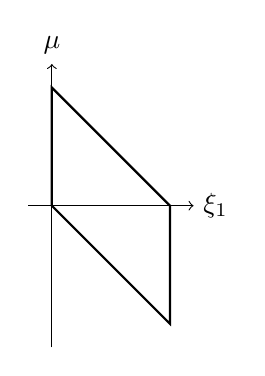
\begin{tikzpicture}[scale=1.5]
\path[draw,->] (-.2,0) -- (1.2,0) node [anchor = west] {$\xi_1$};
\path[draw,->] (0,-1.2) -- (0,1.2) node [anchor = south] {$\mu$};
\path [draw, thick] (0,0) -- (1,-1) -- (1,0) -- (0,1) -- cycle;
\end{tikzpicture}

The order of integration in the first group can be changed as
%
\begin{equation}
\int_{0}^{1} \td \xi_1
\int_{-\xi_1}^{1-\xi_1} \td \mu
=
\int_{-1}^{0} \td \mu
\int_{-\mu}^{1} \td \xi_1
+
\int_{0}^{1} \td \mu
\int_{0}^{1-\mu} \td \xi_1
=
\int_{-1}^{1} \td \mu
\int_{\max(-\mu,0)}^{\min(1-\mu,1)} \td \xi_1
\end{equation}
%
Summarising the above, the total integral can be written as
%
\begin{equation}
\int_{-1}^{1} \td \mu
\int_{0}^{1} \td \xi_2
\int_{0}^{1} \td \eta_2
\int_{\max(-\mu,0)}^{\min(1-\mu,1)} \td \xi_1
\, f(\bm{\xi}-\bm{\eta})
\end{equation}
%
where the outermost three integrals are defined over a brick domain and contain a point singulartiy in the origin, while the innermost integral is regular.

The brick integral with the point singularity is evaluated by splitting the brick domain into six Duffy tetrahedrons defined by the singular point and a non-adjacent face, as shown below. This integration scheme cancels the point singularity like geexci.

\tdplotsetmaincoords{70}{125}
\begin{tikzpicture}[tdplot_main_coords,scale=1.5]
\draw[->] (0,0,0) -- (1.2,0,0) node[anchor=north east]{$\mu$};
\draw[->] (0,0,0) -- (0,1.2,0) node[anchor=north west]{$\xi_2$};
\draw[->] (0,0,0) -- (0,0,1.2) node[anchor=south]{$\eta_2$};
\path [draw, fill] (0,0,0) circle (.1);
\path [draw, thick] (0,0,0) -- (1,0,0) -- (1,1,0) -- (0,1,0) -- (-1,1,0) -- (-1,0,0) -- cycle;
\path [draw, thick] (0,0,1) -- (1,0,1) -- (1,1,1) -- (0,1,1) -- (-1,1,1) -- (-1,0,1) -- cycle;
\path [draw, thick] (0,0,0) -- (0,0,1) -- (0,1,1) -- (0,1,0) -- cycle;
\path [draw, thick] (1,0,0) -- (1,0,1) -- (1,1,1) -- (1,1,0) -- cycle;
\path [draw, thick] (-1,0,0) -- (-1,0,1) -- (-1,1,1) -- (-1,1,0) -- cycle;

\path [draw] (0,0,0) -- (-1,1,0);
\path [draw] (0,0,0) -- (1,1,0);
\path [draw] (0,0,0) -- (0,1,1);
\path [draw] (0,0,0) -- (1,0,1);
\path [draw] (0,0,0) -- (-1,0,1);
\path [draw] (0,0,0) -- (1,1,1);
\path [draw] (0,0,0) -- (-1,1,1);
\end{tikzpicture}


\subsection{Edge match with two triangles}


\tdplotsetmaincoords{70}{125}
\begin{tikzpicture}[tdplot_main_coords,scale=1.5]
\draw[->] (0,0,0) -- (1.2,0,0) node[anchor=north east]{$\mu$};
\draw[->] (0,0,0) -- (0,1.2,0) node[anchor=north west]{$\xi_2$};
\draw[->] (0,0,0) -- (0,0,1.2) node[anchor=south]{$\eta_2$};
\path [draw, fill] (0,0,0) circle (.1);
\path [draw, thick] (0,0,0) -- (1,0,0) -- (0,1,0) -- (-1,1,0) -- (-1,0,0) -- cycle;
\path [draw, thick] (0,0,1) -- (1,0,1) -- (0,1,1) -- (-1,1,0) -- (-1,0,0) -- cycle;
\path [draw, thick] (0,0,0) -- (0,0,1) -- (0,1,1) -- (0,1,0) -- cycle;
\path [draw, thick] (1,0,0) -- (1,0,1);
\end{tikzpicture}




\end{document}

